% This is samplepaper.tex, a sample chapter demonstrating the
% LLNCS macro package for Springer Computer Science proceedings;
% Version 2.21 of 2022/01/12
%

\documentclass[runningheads]{llncs}
%
\usepackage[T1]{fontenc}
\usepackage{pdfpages}
\usepackage{tabularx}
\usepackage{booktabs}
\newcolumntype{Y}{>{\raggedright\arraybackslash}X}

% T1 fonts will be used to generate the final print and online PDFs,
% so please use T1 fonts in your manuscript whenever possible.
% Other font encondings may result in incorrect characters.
%
\usepackage{graphicx}
% Used for displaying a sample figure. If possible, figure files should
% be included in EPS format.
%
% If you use the hyperref package, please uncomment the following two lines
% to display URLs in blue roman font according to Springer's eBook style:
%\usepackage{color}
%\renewcommand\UrlFont{\color{blue}\rmfamily}
%\urlstyle{rm}
%
\begin{document}
%
\title{Knowledge Elicitation and Ontology-Based Visualization of Business Ecosystems: A Case Study from the 
Green Energy Ecosystem}
%
%\titlerunning{Abbreviated paper title}
% If the paper title is too long for the running head, you can set
% an abbreviated paper title here
%
\author{Alican Tüzün\inst{1,2}\orcidID{0009-0009-8017-5487} \and
Georgios Meditskos\inst{1}\orcidID{0000-0003-4242-5245}
}
%
\authorrunning{F. Author et al.}
% First names are abbreviated in the running head.
% If there are more than two authors, 'et al.' is used.
%
\institute{School of Informatics, Aristotle University of Thessaloniki, Thessaloniki, Greece\and
Josef Ressel Centre for Data-Driven Business Model Innovation, University of Applied Sciences Upper Austria, 
Wehrgrabengasse 1-4, 4400, Steyr, Austria
\email{lncs@springer.com}\\
\url{http://www.springer.com/gp/computer-science/lncs}}
%
\maketitle              % typeset the header of the contribution
%
\begin{abstract}
The abstract should briefly summarize the contents of the paper in
150--250 words.

\keywords{Business Ecosystem  \and Knowledge Representation \and Symbolic Artifical Intelligence.}
\end{abstract}
%
%
%
\section{Introduction}

\subsection{Challange}
\subsection{Business ecosystems}
\subsection{Green Energy Ecosystem}
\subsection{Research Question}
\begin{center}
\textit{How can organizational interactions in the wind energy ecosystem 
systematically captured and translated into structured formal knowledge representations to enable data-driven decisions?}
\end{center}

\section{Methology}

\subsection{Semi-Structured Survey}

\begin{table}[ht]
    \centering
    \caption{Relationships and Theoretical Foundations}
    \label{tab:relationships}
    \begin{tabularx}{\textwidth}{lYY}
    \toprule
    \textbf{Relationship Type} & \textbf{Theoretical Foundation} & \textbf{Logical Charecteristics} \\
    \midrule
    Product \& Service Delivery & 
    Supply Chain Management (Chopra \& Meindl, 2016); 
    Value Chain Analysis (Porter, 1985); 
    Business Ecosystems (Adner, 2017) & 
    Irreflexive, Transitive \\
    \addlinespace
    
    Payment & 
    Business Model Ontology (Osterwalder \& Pigneur, 2005); 
    Value Network Analysis (Allee, 2008); 
    Input-Output Economics (Leontief, 1986) & 
    Irreflexive \\
    \addlinespace
    
    Data & 
    Knowledge-Based View (Grant, 1996); 
    Digital Ecosystem Theory (Tiwana, 2013) &
    Irreflexive \\
    \addlinespace
    
    Information & 
    Knowledge-Based View (Grant, 1996) & 
    Irreflexive \\
    \addlinespace
    
    Collaboration & 
    Resource-Based View (Barney, 1991) & 
    Irreflexive, Symmetric \\
    \addlinespace
    
    Conflict & 
    Stakeholder Theory (Freeman, 1984) & 
    Irreflexive,ASymmetric \\
    \addlinespace
    
    Competition & 
    Porter's Five Forces (Porter, 1979) & 
    Irreflexive, Symmetric \\
    \addlinespace
    
    Coopetition (Implicit) & 
    Coopetition Theory (Brandenburger \& Nalebuff, 1996) & 
    Irreflexive \\
    \bottomrule
    \end{tabularx}
    \smallskip
    \end{table}

\subsection{OWL2}

\subsection{Ontological Commitments}

\begin{itemize}
    \item \textbf{ClassAssertion }
    \item \textbf{ClassHierarchyAssertion}
    \item \textbf{ClassDisjointnessAssertion}
    \item \textbf{ObjectPropertyAssertion}
    \item \textbf{PropertyCharacteristicAssertions}
    \item \textbf{Methodological Limitations}
\end{itemize}

\subsection*{Visualization}

\subsubsection{js}

\subsubsection{d3.js}

Methodological Limitations


\section{Results\&Discussion}

\subsection{Survey Results\&Discussion}
\subsection{Ontology Development}
\subsection{Information Retrieval with Sparql}
\subsection{Visualization Results}

\section{Conclusion}

\appendix{Data}
\appendix{Source Code for Ontology}
\appendix{Source Code for Visualization}

\bibliographystyle{splncs04}
\bibliography{reference}

\appendix

\section{Survey}
%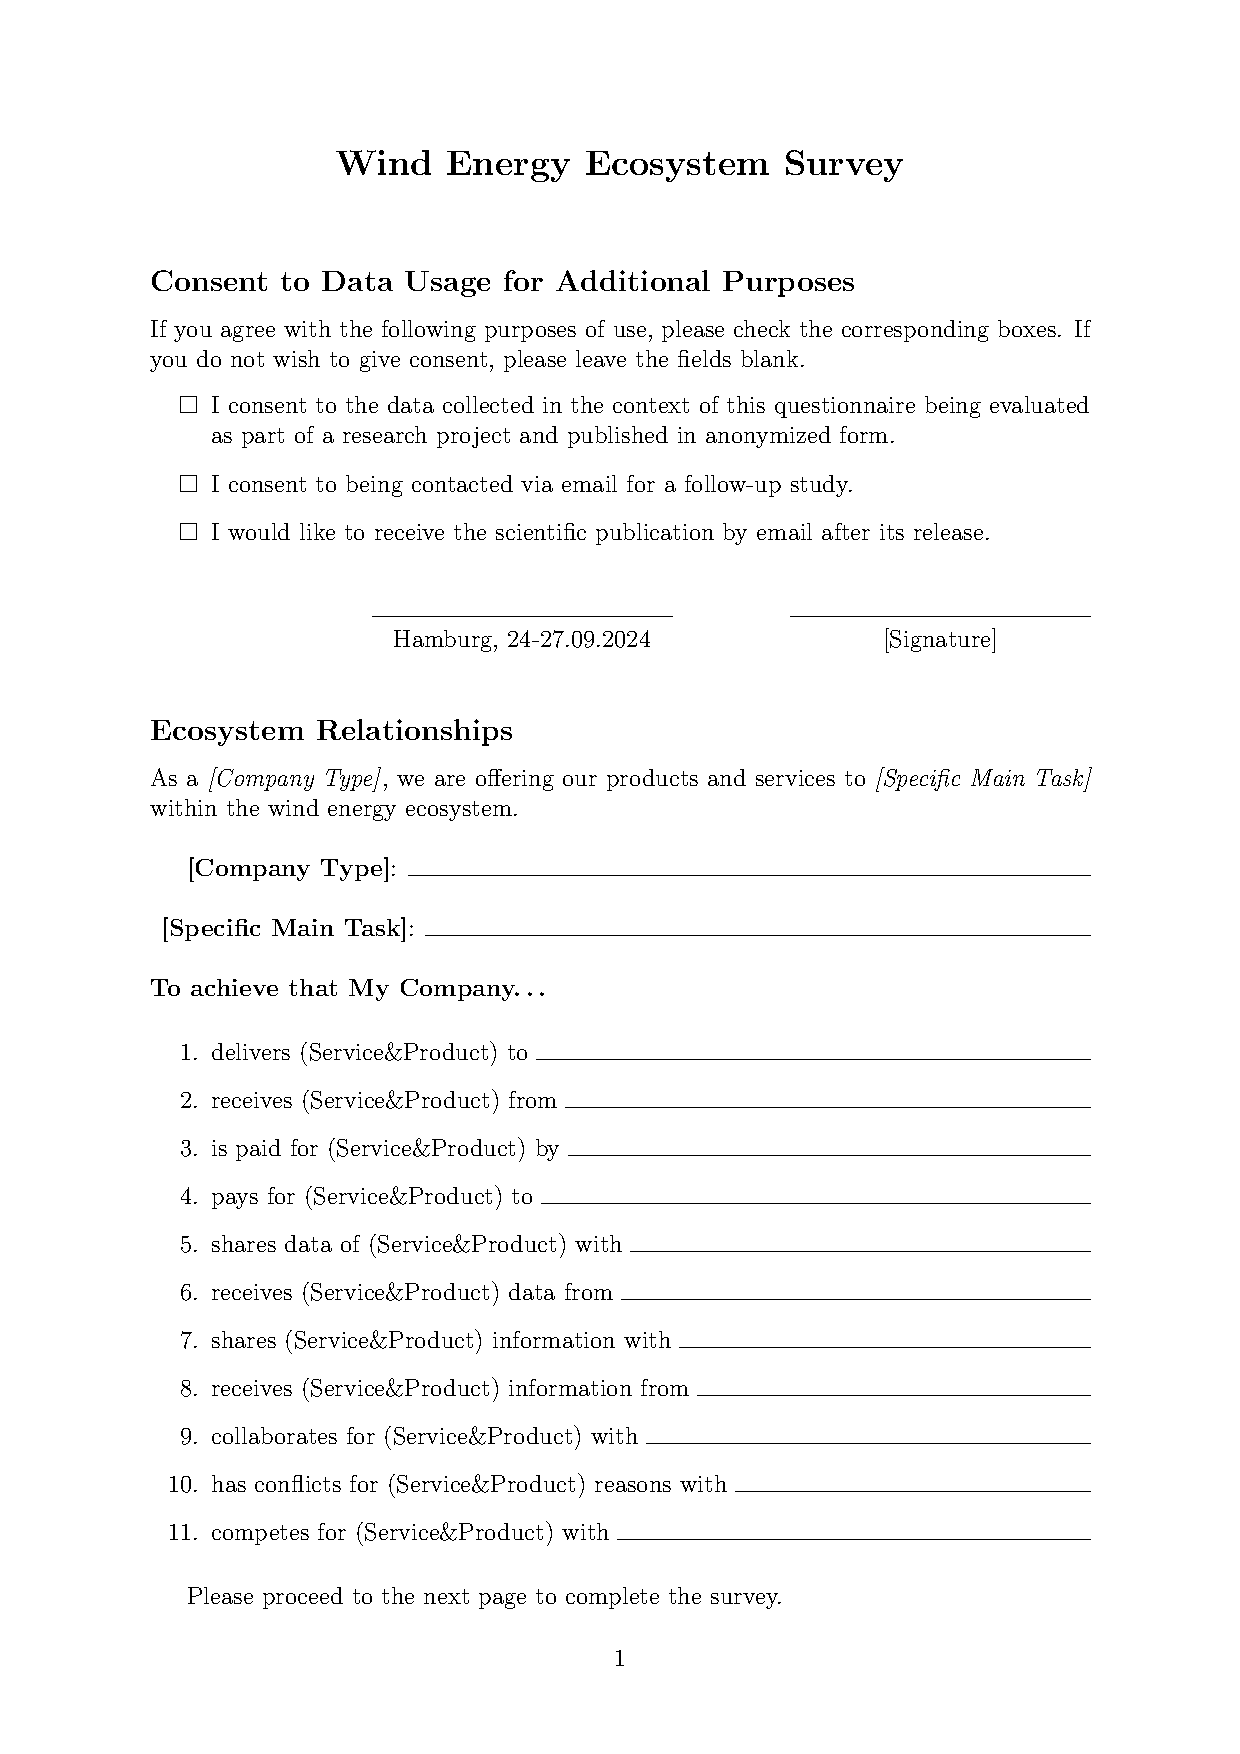
\includepdf[pages=-]{survey.pdf}


\end{document}

